\chapter{Modelos epidemiológicos}

\section{Modelos compartimentales}

Para modelar la propagación de enfermedades infecciosas, es muy habitual utilizar modelos compartimentales basados en ecuaciones diferenciales. Estos pueden ser utilizados para predecir y comprender situaciones epidemiológicas, ayudar a la toma de decisiones y simular situaciones hipotéticas así como también se pueden utilizar para estimar parámetros. Su origen se remonta a los años 20 del siglo pasado y suele atribuirse a \cite{Kermack1927}. Estos consisten en modelar la población distinguiendo subpoblaciones de acuerdo a categorías epidemiológicas. Por ejemplo, el emblemático modelo SIR, distingue a las subpoblaciones susceptible ($S$), infectada ($I$) y recuperada ($R$). Este se puede expresar mediante el siguiente sistema de ecuaciones diferenciales,
\begin{align}
    \frac{\partial S}{\partial t} &= -\beta \frac{SI}{N}\\
    \frac{\partial I}{\partial t} &= \beta \frac{SI}{N} - \gamma I \\
    \frac{\partial R}{\partial t} &= \gamma I
\end{align}
Estas ecuaciones suponen una población constante de tamaño $N$: notemos que las ecuaciones suman 0 por lo que la población total se mantiene. La velocidad con que los individuos susceptibles se infectan es proporcional a la cantidad total de susceptibles, $S$ y a la proporción de infectados de la población $\frac{I}{N}$. La constante de proporcionalidad $\beta$ es llamada la tasa de infección y cuantifica la transmisibilidad de la enfermedad. Por su parte, la velocidad con que los infectados se recuperan es proporcional a la cantidad de infectados y la constante de proporcionalidad $\gamma$ es llamada tasa de recuperación.

El modelo SIR, aunque sencillo, merece mención pues tiene los elementos básicos con los que se puede construir un modelo compartimental. Como vimos, la entrada y salida de cada compartimento se describe con una ecuación diferencial y con esta idea se pueden diseñar distintas estructuras de subpoblaciones para describir las situaciones que se deseen modelar. Es común ver en este tipo de modelos la subpoblación de los decesos $D$ que permite distinguir a la porción de la población que muere a causa de la enfermedad, o la subpoblación de los expuestos $E$ se suele ver en modelos para enfermedades virales en que las personas se infectan e incuban el virus sin ser infecciosas antes de pasar al compartimento $I$. De esta manera tenemos modelos como el SEIRD que considera estas subpoblaciones, o el SIS que no tiene en cuenta una categoría de recuperados que no contagia sino que las personas, al curarse de la enfermedad vuelven a ser susceptibles. Otros modelos como el SIRV, consideran el comprtimento de vacunados $V$ que pasan a ser inmunes al contagio. En, general podemos distinguir 3 tipos distintos de compartimentos: aquellos que actúan de fuente, es decir que solo decrecen o se mantienen, y por lo tanto los términos en las ecuaciones diferenciales son sólo negativos, los compartimentos intermedios, cuyas ecuaciones incluyen términos positivos y negativos y finalmente los compartimentos que actúan de resumidero, es decir que sólo crecen o se mantienen los cuales sólo incluyen términos positivos. Por ejemplo, en el modelo SIR el compartimento $S$ actúa a modo de fuente, $I$ es un compartimento intermedio y $R$ actúa de resumidero. Típicamente las trayectorias de las fuentes tienen una forma sigmoidea decreciente y las de los resumideros son sigmoideas decrecientes mientras que los compartimientos intermedios suelen exhibir un comportamiento con forma de campana. En la figura \ref{fig:sir_example} se puede observar esto en las trayectorias generadas por un modelo SIR.

\begin{figure}[h]
    \centering
    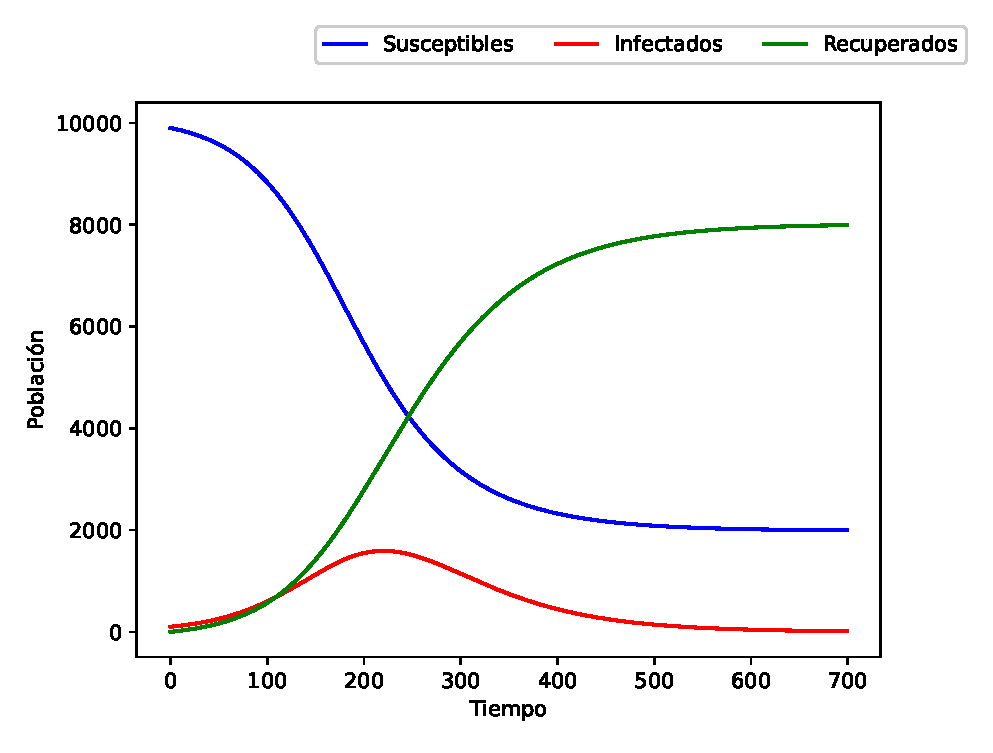
\includegraphics[width=0.75\textwidth]{sir_example.eps}
    \caption{}
    \label{fig:sir_example}
\end{figure}

Los modelos compartimentales pueden además incluir otras características como varaibles espaciales acopladas a términos de difusión en las ecuaciones que dan cuenta de la dispersión territorial de las enfermedades. También se utiliza estratificación por edades para diferenciar el efecto de la enfermedad en distintos sectores de la población y codificar el contacto entre los distintos rangos etarios. También se puede modelar la espacialidad a través de la determinación de áreas, por ejemplo barrios en una ciudad, cada una con sus propias subpoblaciones de susceptibles, infectados etc. y describiendo la interacción entre estos lugares.

\section{Inferencia en modelos epidemiológicos}
EnkF con estimación de R0

Ionides Shaman Karspeck Evensen (ES-EMDA)

\section{Estimación de errores en modelos compartimentales}
online EM

\section{Modelos basados en agentes}
\subsection{Modelo SEIHRD}
